% MAMA-SYNTH 2026 Workshop Paper % Springer LNCS Template - Double-blind submission % Deadline: July 15, 2026
\documentclass[runningheads,a4paper]{llncs}
\usepackage{graphicx}
\usepackage{amsmath}
\usepackage{amssymb}
\usepackage{booktabs}
\usepackage{multirow}
\usepackage{xcolor}
\usepackage{hyperref}

% Float and spacing settings for 8-page fit
\renewcommand{\topfraction}{0.85}
\renewcommand{\bottomfraction}{0.85}
\renewcommand{\textfraction}{0.15}
\renewcommand{\floatpagefraction}{0.75}
\setlength{\textfloatsep}{10pt plus 2pt minus 4pt}
\setlength{\floatsep}{10pt plus 2pt minus 4pt}
\setlength{\intextsep}{10pt plus 2pt minus 4pt}
\setlength{\abovecaptionskip}{6pt}
\setlength{\belowcaptionskip}{4pt}

% Allow TeX slightly more slack before declaring an overfull line. Needed
% because several long hyphenated terms (e.g. "multi-scale enhancement
% consistency") otherwise overrun the measure by 1-5pt.
\setlength{\emergencystretch}{1em}

\begin{document}
\title{Tumor-Aware Conditional Pix2PixHD with Per-Image Normalization for Virtual Contrast Enhancement in Breast MRI}
\titlerunning{Tumor-Aware Conditional GAN for Virtual Contrast Enhancement}
\author{Hong Jiang \and Zhikai Yang \and Rodrigo Moreno}
\authorrunning{H. Jiang et al.}
\institute{KTH Royal Institute of Technology, Stockholm, Sweden\\
\email{\{hongjia,zhikai,rodmore\}@kth.se}}
\maketitle

\begin{abstract}
Dynamic contrast-enhanced MRI (DCE-MRI) is essential for breast cancer diagnosis but requires gadolinium-based contrast agents that pose safety and accessibility concerns. We present a conditional generative adversarial network for synthesizing post-contrast breast MRI from pre-contrast T1-weighted acquisitions. Our method introduces two key contributions: (1) per-image z-score normalization that eliminates cross-scanner intensity variation, improving perceptual similarity by 25\%; and (2) a predicted tumor mask as conditional input that provides the generator with an explicit spatial prior for enhancement localization, improving downstream segmentation Dice by 14\%. We additionally isolate the multi-scale enhancement consistency (MSEC) loss inherited from our earlier multi-parametric work and find it redundant once these two components are present. On our internal validation set, the method achieves a tumor-region SSIM of 0.509, a downstream segmentation Dice of 0.624, and a 95th-percentile Hausdorff distance (HD95) of 69.4, demonstrating that tumor-aware conditional synthesis can produce clinically meaningful virtual contrast enhancement.
\end{abstract}
\keywords{Virtual contrast enhancement \and Breast DCE-MRI \and Conditional GAN \and Image-to-image translation \and Per-image normalization}

% ============================================================================
\section{Introduction}
% ============================================================================
Dynamic contrast-enhanced MRI (DCE-MRI) plays a central role in breast cancer screening, diagnosis, and treatment monitoring~\cite{mann2019breast}, but the gadolinium-based contrast agents (GBCAs) it requires raise concerns over patient safety --- including nephrogenic systemic fibrosis and gadolinium deposition in neural tissue~\cite{kanda2014gadolinium} --- as well as examination time, cost, and pharmaceutical waste.

Virtual contrast enhancement (VCE) synthesizes post-contrast images from non-contrast acquisitions, and the MAMA-SYNTH 2026 challenge~\cite{mamasynth2026} provides a standardized benchmark for it. Two difficulties dominate. First, MRI intensities are not standardized across scanners, institutions, and protocols, producing inter-patient variation that confounds learning-based methods. Second, enhancement is spatially heterogeneous --- tumors enhance focally while normal tissue shows subtle background uptake --- so a synthesis model must both localize and modulate it.

We propose a conditional Pix2PixHD framework addressing both. Our contributions are (1) \textbf{per-image z-score normalization}, which maps each image into a scanner-invariant canonical space using its own breast-region statistics, and (2) a \textbf{tumor-aware conditional input}, which supplies a predicted tumor mask as an extra channel so the generator receives explicit spatial information about where enhancement should occur. Both are trained alongside the multi-scale enhancement consistency (MSEC) loss~\cite{yang2026miccai}, which we inherit unchanged from our earlier multi-parametric work and, in an ablation reported below, find to be redundant in this single-modality setting.

\paragraph{Related work.}
GAN-based image-to-image translation is widely used for medical image synthesis, with Pix2PixHD~\cite{wang2018pix2pixHD} introducing multi-scale discriminators for high-resolution outputs. The MSEC loss was introduced in our earlier work~\cite{yang2026miccai} for DCE-MRI synthesis from multi-parametric inputs; we carry it over unchanged to the harder single-modality (T1w-only) setting. Our contributions relative to that work are per-image normalization for multi-institutional data and predicted tumor masks as spatial conditioning.

% ============================================================================
\section{Method}
% ============================================================================
\subsection{Overview}
Given a pre-contrast T1-weighted slice $x \in \mathbb{R}^{H \times W}$, we obtain a binary breast mask $m_b$ and a predicted tumor mask $m_t$ from trained segmentation models, normalize $x$ to a canonical intensity space using breast-region statistics, synthesize the post-contrast image from the three-channel input $[x_{\text{norm}}, m_b, m_t]$, and de-normalize and composite the result with the original background. Test-time augmentation (TTA) is applied at inference. Figure~\ref{fig:pipeline} shows the training pipeline.

\begin{figure}[t]
\centering
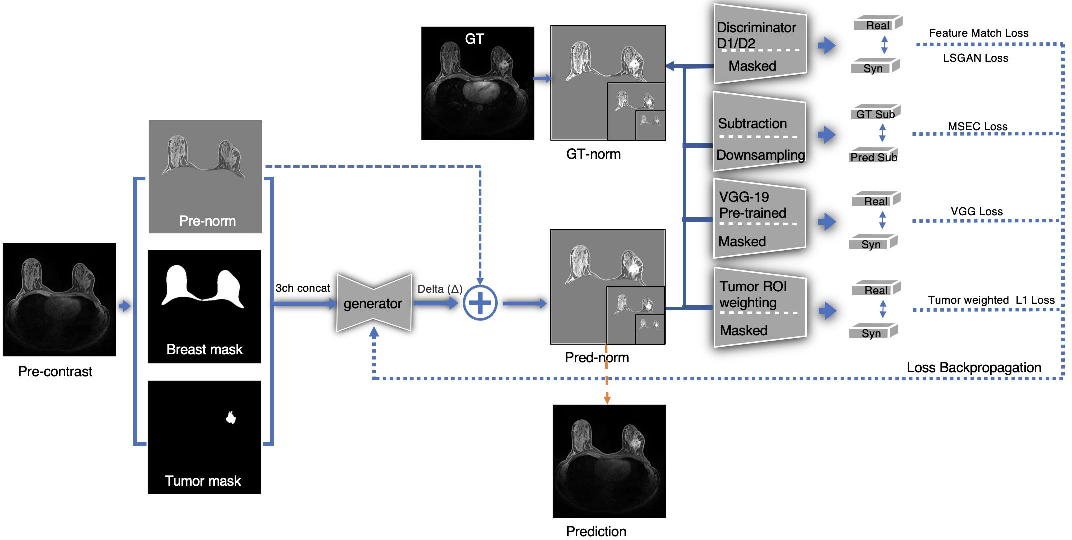
\includegraphics[width=0.92\textwidth]{figures/pipeline.pdf}
\caption{Training pipeline. The pre-contrast input is per-image normalized and concatenated with breast and tumor masks to form a 3-channel input. The generator predicts a residual enhancement map supervised by five masked losses: GAN, feature matching, VGG perceptual, MSEC, and tumor-weighted L1.}
\label{fig:pipeline}
\end{figure}

\subsection{Per-Image Z-Score Normalization}
The challenge data are supplied in a global z-score space, normalized with dataset-level statistics. This removes absolute intensity offsets but leaves substantial inter-scanner variation (Table~\ref{tab:dataset}), so we apply a second, per-image normalization using each image's own breast-region statistics:
\begin{equation}
x_{\text{norm}} = \frac{x - \mu_{\text{img}}}{\sigma_{\text{img}}}, \qquad
y_{\text{norm}} = \frac{y - \mu_{\text{img}}}{\sigma_{\text{img}}}
\end{equation}
where $\mu_{\text{img}}$ and $\sigma_{\text{img}}$ are computed over breast foreground pixels ($m_b > 0$) of the \emph{pre-contrast} image, and background pixels are set to zero. Note that the post-contrast target $y$ is deliberately normalized with the same pre-contrast statistics: this places input and target in a common canonical space, so the residual formulation below operates on enhancement differences in a scanner-invariant manner. At inference, de-normalization restores the original intensity, $\hat{y} = G(x_{\text{norm}}, m_b, m_t) \cdot \sigma_{\text{img}} + \mu_{\text{img}}$.

\subsection{Tumor-Aware Conditional Input}
A standard 1-channel generator must learn both \textit{where} and \textit{how much} to enhance. We decouple these by providing a predicted tumor mask as spatial prior. A 2D nnU-Net~\cite{isensee2021nnunet} trained on pre-contrast images predicts $m_t$, which is concatenated as the third input channel:
\begin{equation}
\hat{y}_{\text{norm}} = G([x_{\text{norm}}, m_b, m_t])
\end{equation}

This allows the generator to focus on enhancement intensity rather than localization.

\paragraph{Provenance and patient-level separation of the segmentation models.}
The two conditioning masks have different provenance, and neither can leak test-set information. The breast segmentor $m_b$ is a 2D nnU-Net obtained by pseudo-label distillation from an external teacher on public data only: the BreastDivider dataset (\texttt{Bubenpo/BreastDividerDataset}) ships segmentations produced by the 3D BreastDivider model (\texttt{ykirchhoff/Bre\-astDividerModel})~\cite{rokuss2025breastdivider}, and we use those teacher outputs unmodified as targets for a 2D student trained on mid-axial slices with labels binarized to breast versus background. It never observes a MAMA-SYNTH image, so leakage is excluded by construction rather than by a split. The tumor segmentor $m_t$ is trained on our own data, where separation does matter: its nnU-Net dataset was built exclusively from the 9,504 train-split slices used for the GAN, so none of the 60 held-out test patients contribute a slice. The patient-level separation asserted for the evaluation segmenter (Sec.~\ref{subsec:experiment_setting}) therefore holds identically here, and the conditioning input is never informed by test-patient annotations. On its own validation fold (1,901 slices, nnU-Net's internal split) it reaches a foreground Dice of 0.767.

As a further check against annotation leakage, we re-ran the final configuration with ground-truth tumor masks substituted for the predicted ones at test time. Dice moves only from 0.624 to 0.627, and MSE, LPIPS and FRD are essentially unchanged (1.127, 0.123, 27.04). The predicted masks therefore already realize almost all of the benefit that perfect localization could provide, leaving a headroom of 0.003 Dice. Two things follow. The 14\% gain from tumor conditioning (rows (2)--(3) of Table~\ref{tab:merged_results}) cannot stem from privileged access to test annotations, since supplying those annotations outright changes almost nothing. And the design tolerates the imperfect masks that a 0.767-Dice segmentor produces, which is what makes the approach practical.

\subsection{Network Architecture}
We adapt the GlobalGenerator of Pix2PixHD~\cite{wang2018pix2pixHD}: four strided convolutions (ngf=64) compress the $512 \times 512$ three-channel input to $32 \times 32$, 12 residual blocks model the enhancement, and four transpose convolutions decode back to full resolution, with Instance Normalization throughout. The generator runs in residual mode, predicting only the enhancement difference $\Delta$ so that $\hat{y}_{\text{norm}} = x_{\text{norm}} + \Delta$; this preserves anatomy by construction and avoids spending capacity on reproducing the static background. The discriminator is a multi-scale PatchGAN~\cite{wang2018pix2pixHD} with two branches (full and half resolution, 3 layers each).

\subsection{Training Strategy}
\paragraph{Dataset and preprocessing.}
The primary cohort comes from MAMA-MIA~\cite{muller2022mama} as provided by the challenge~\cite{mamasynth2026}. For orientation consistency with the official test set we keep only axial acquisitions (DUKE, ISPY2) and drop the sagittal cohorts (DUKE1, ISPY1, NACT), supplementing with three public cohorts for generalization: YUNNAN~\cite{yunnan2024}, AMBL~\cite{ambl2024}, and LA-Breast~\cite{labreast2023}. To keep the pixel-wise supervisory signal clean, we estimate pre-to-post translation by phase correlation and discard patients displaced by more than 3 pixels (81 ISPY2 patients, i.e.\ all of their slices). For each patient we take the peak-enhancement phase (highest mean tumor intensity) and the axial slice with the largest tumor cross-section, plus its four neighbours ($\pm 1, \pm 2$) to enrich diversity while preserving local coherence --- five slices per volume, 9,504 training slices in total. Images and masks are resampled to $512 \times 512$ with bilinear and nearest-neighbour interpolation respectively.

\paragraph{Loss Function.}
All loss terms are spatially restricted to the breast parenchyma via $m_b$, so no capacity is spent on clinically irrelevant background. The joint objective is
\begin{equation}
\mathcal{L}_G = \lambda_{GAN}\mathcal{L}_{GAN} + \lambda_{feat}\mathcal{L}_{feat} + \lambda_{VGG}\mathcal{L}_{VGG} + \lambda_{MSEC}\mathcal{L}_{MSEC} + \lambda_{tumor}\mathcal{L}_{tumor}
\end{equation}
where $\mathcal{L}_{GAN}$ is a least-squares (LSGAN) term over the two PatchGAN scales encouraging high-frequency texture, $\mathcal{L}_{feat}$ is the $L_1$ distance between intermediate discriminator features of real and synthesized images (stabilizing training), and $\mathcal{L}_{VGG}$ is a VGG-19 perceptual loss. The \textbf{multi-scale enhancement consistency (MSEC)} loss~\cite{yang2026miccai} acts on subtraction maps to enforce hemodynamic plausibility,
\begin{equation}
\mathcal{L}_{MSEC} = \sum_{s=1}^{S} | D_s(\hat{y}_{\text{norm}} - x_{\text{norm}}) - D_s(y_{\text{norm}} - x_{\text{norm}}) |_1
\end{equation}
with $D_s$ downsampling to scale $s$ ($S=3$: $1\times$, $\frac{1}{2}\times$, $\frac{1}{4}\times$), capturing both focal and global enhancement. We adopt it unchanged from~\cite{yang2026miccai}, weighting included, and isolate its contribution via the $\lambda_{MSEC}=0$ ablation in Section~\ref{subsec:results}. Finally, since tumors occupy a small fraction of the breast, a \textbf{tumor-weighted} term counters this class imbalance with focused $L_1$ supervision, $\mathcal{L}_{tumor} = | (\hat{y}_{\text{norm}} - y_{\text{norm}}) \odot m_t |_1$.

\paragraph{Data Augmentation.}
We apply additive Gaussian noise ($\sigma \sim U[0.02, 0.05]$) and random horizontal flipping during training.

\paragraph{Optimization.}
We train for 200 epochs with batch size 16, learning rate $3\times10^{-4}$ with linear decay after epoch 100, using Adam optimizer. The hyperparameter $\lambda_{GAN}=1$, $\lambda_{feat}=10$, $\lambda_{VGG}=10$, $\lambda_{MSEC}=50$, $\lambda_{tumor}=10$.

\subsection{Inference Pipeline}
At test time (Fig.~\ref{fig:inference_pipeline}) we predict $m_b$ and $m_t$ with the two nnU-Nets described above, normalize per image, and synthesize from the 3-channel input using horizontal-flip TTA: the generator is run on the original and the flipped input, the second output is flipped back, and the two are averaged to reduce directional bias. After de-normalization the result is blended with the original background,
\begin{equation}
y_{\text{out}} = m_b^{\text{soft}} \cdot \hat{y} + (1 - m_b^{\text{soft}}) \cdot x
\end{equation}
where $m_b^{\text{soft}}$ is the breast mask smoothed by a Gaussian filter ($\sigma = 5$ pixels) to remove boundary artifacts. Total inference time is $\sim$3\,s per slice on an NVIDIA T4 GPU.

\begin{figure}[t]
\centering
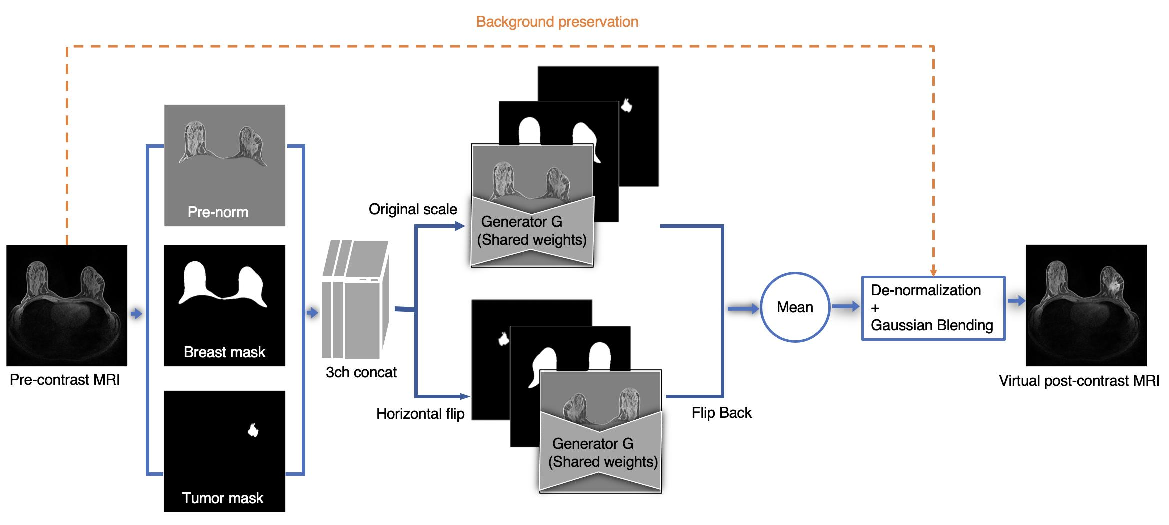
\includegraphics[width=0.74\textwidth]{figures/inference.pdf}
\vspace{-3mm}
\caption{Inference pipeline. The pre-contrast MRI is segmented, normalized, and concatenated into a 3-channel input. Horizontal-flip TTA averages two forward passes to cancel synthesis noise. The output is de-normalized and blended with the original background via a Gaussian-smoothed breast mask ($\sigma = 5$ pixels).}
\label{fig:inference_pipeline}
\vspace{-4mm}
\end{figure}

% ============================================================================
\section{Experiments}
% ============================================================================
\subsection{Experiment Setting}
\label{subsec:experiment_setting}
We evaluate on an internal test set comprising 299 slices from 60 patients held out from three institutions: DUKE (55 slices from 11 patients), ISPY2 (219 slices from 44 patients), and YUNNAN (25 slices from 5 patients), representing approximately 5\% of each dataset. The split was strictly performed at the patient level. AMBL and LA-Breast are used only for training, as their tumor annotations are approximate (enhancement-based thresholding and elliptical ROI fitting), making them unsuitable for segmentation-based evaluation. Table~\ref{tab:dataset} summarizes the training data composition.

\begin{table}[t] 
\centering 
\caption{Training and testing data composition. Mean/Std computed over breast foreground pixels in global z-score space.} 
\label{tab:dataset} 
\begin{tabular}{lccccc} 
\toprule 
Dataset & Train slices & Test slices & Resolution & Mean (avg $\pm$ std) & Std (avg $\pm$ std) \\ 
\midrule 
ISPY2 & 4267 & 219 & 256--384 & $0.29 \pm 0.56$ & $0.97 \pm 0.72$ \\ 
AMBL & 2462 & -- & 512 & $-0.30 \pm 0.10$ & $0.30 \pm 0.16$ \\ 
LA-Breast & 1179 & -- & 448--480 & $-0.40 \pm 0.01$ & $0.12 \pm 0.01$ \\ 
DUKE & 1124 & 55 & 448--512 & $0.06 \pm 0.48$ & $0.87 \pm 0.78$ \\ 
YUNNAN & 472 & 25 & 896 & $-0.33 \pm 0.05$ & $0.23 \pm 0.07$ \\ 
\midrule 
\textbf{Total} & \textbf{9504} & \textbf{299} & & & \\ 
\bottomrule 
\end{tabular} 
\end{table}

\paragraph{Diffusion baseline.}
The SUB-DDPM numbers in Table~\ref{tab:merged_results} are \emph{not} taken from the challenge organizers' leaderboard: they come from our own adaptation of the subtraction-based conditional diffusion model of Ibarra et al.~\cite{ibarra2025diffusion}, evaluated on the same 299-slice test set used throughout this work. We reuse the authors' released implementation unchanged in its essentials --- the lightweight \texttt{ConditionalUNet} (8.4M parameters), the $x_0$-prediction formulation with a cosine$^2$ noise schedule, the subtraction target $\mathrm{clip}((y-x)/0.5,-1,1)$, and the composite objective of $0.3\times$MAE $+\ 0.6\times$VGG perceptual $+\ 0.15\times$total variation $+\ 0.05\times$MSE. It was trained for 100 epochs with exponential moving averaging, and we report the best checkpoint sampled with 50 denoising steps (250 training timesteps). Our single substantive departure is the input pipeline, discussed next.

Two factors are important for interpreting the size of the reported gap. First, the two models were not trained on identical data volumes: our generator uses 9,504 training slices, whereas this baseline was trained on 1,194, so the comparison is not compute- or data-matched. Second, and more informative, the method's preprocessing assumptions are incompatible with the intensity representation mandated by this benchmark. The original pipeline min-max normalizes each slice to $[0,1]$ before mapping to $[-1,1]$, so the full dynamic range of every slice is preserved and the $\mathrm{clip}((y-x)/0.5,-1,1)$ target rarely saturates. The challenge instead supplies globally z-scored volumes, which we map to $[-1,1]$ by clipping at $\pm 3$; in a test cohort containing intensities up to $\approx 18$, this truncates the bright voxels that carry the enhancement signal, and the subsequent $\times 2$ scaling of the subtraction target saturates whatever survives. The resulting attenuation is a plausible explanation for the very low $\text{SSIM}_{\text{tumor}}$ and high MSE. We therefore read this row not as evidence against the published method or against conditional diffusion in general, but as an indication that per-slice min-max normalization is load-bearing for this family of models and does not transfer directly to a globally z-scored benchmark.

Evaluation metrics include: mean squared error (MSE), learned perceptual image patch similarity (LPIPS)~\cite{zhang2018lpips}, structural similarity in the tumor region ($\text{SSIM}_{\text{tumor}}$)~\cite{wang2004image}, Fr\'{e}chet radiomics distance (FRD), and downstream segmentation quality (Dice coefficient, 95th-percentile Hausdorff distance, HD95) using an independent nnU-Net.

\subsection{Quantitative Results and Ablation Study}
\label{subsec:results}

\begin{table}[!t]
\centering
\caption{Comparison with diffusion baseline and cumulative ablation on the internal test set (299 slices from 60 patients). Rows (1)--(4) all include the MSEC loss; row (5) removes it from the final configuration. Row (4) is our reported configuration (see text); row (5) scores better on SSIM and FRD. Best values in \textbf{bold}.}
\label{tab:merged_results}
\begin{tabular}{lcccccc}
\toprule
Method / Configuration & MSE $\downarrow$ & LPIPS $\downarrow$ & SSIM $\uparrow$ & FRD $\downarrow$ & Dice $\uparrow$ & HD95 $\downarrow$ \\
\midrule
\textit{Diffusion Baseline} & & & & & & \\
SUB-DDPM (50 steps) \cite{ibarra2025diffusion} & 3.233 & 0.316 & 0.029 & 30.26 & 0.072 & 419.8 \\
\midrule
\textit{Ours (Ablation Progression)} & & & & & & \\
(1) Global z-score (Baseline) & \textbf{1.101} & 0.157 & 0.394 & 29.66 & 0.493 & 144.9 \\
(2) + Per-image z-score & 1.236 & 0.117 & 0.476 & 28.45 & 0.539 & 125.6 \\
(3) + 3ch conditional (tumor mask) & 1.160 & \textbf{0.116} & 0.492 & 28.46 & 0.614 & 76.0 \\
(4) + Blending \& TTA (full model) & 1.127 & 0.123 & 0.509 & 27.06 & \textbf{0.624} & \textbf{69.4} \\
\midrule
\textit{MSEC ablation} & & & & & & \\
(5) (4) with $\lambda_{MSEC}=0$ & 1.120 & 0.125 & \textbf{0.520} & \textbf{25.83} & \textbf{0.624} & 69.8 \\
\bottomrule
\end{tabular}
\end{table}

\paragraph{Diffusion baseline and component contributions.}
The diffusion baseline scores poorly on this multi-center test set (SSIM 0.029, Dice 0.072, HD95 419.8). As discussed in Section~\ref{subsec:experiment_setting}, we attribute this mainly to the reduced training set and to the mismatch between the method's per-slice min-max normalization and the globally z-scored inputs of this benchmark, not to an inherent limit of conditional diffusion; the original authors report substantially stronger results under their own preprocessing. Our global z-score baseline already outperforms it on every metric.

Among our own components, \textbf{per-image normalization} is what buys perceptual quality: it cuts LPIPS by 25\% (0.157 $\to$ 0.117) and raises SSIM by 21\% (0.394 $\to$ 0.476), the small MSE increase (1.101 $\to$ 1.236) reflecting the familiar trade-off between $L_2$ optimization and perceptual similarity. The \textbf{conditional tumor mask} instead drives localization, improving Dice by 14\% (0.539 $\to$ 0.614) and cutting HD95 by 39\% (125.6 $\to$ 76.0); decoupling spatial search from intensity modeling lets the generator concentrate capacity on the tumor. \textbf{Blending and hflip TTA} add final refinements --- TTA averages out high-frequency noise and soft-boundary blending removes edge artifacts --- reaching SSIM 0.509, Dice 0.624, HD95 69.4. Figure~\ref{fig:qualitative} shows qualitative results across the three cohorts.

\paragraph{MSEC brings no net benefit once normalization and tumor conditioning are in place.}
Rows (1)--(4) all include MSEC, so the progression above does not isolate it. We therefore retrained the full model with $\lambda_{MSEC}=0$, changing no other hyperparameter, and evaluated it through the identical inference and scoring pipeline; as a control, the $\lambda_{MSEC}=50$ weights re-run through that pipeline reproduced row (4) to four decimal places on all six metrics. Removing MSEC (row 5) leaves Dice unchanged (0.6236 vs.\ 0.6236) and \emph{improves} $\text{SSIM}_{\text{tumor}}$ (0.509 $\to$ 0.520, paired Wilcoxon $p=1\times10^{-4}$, 178/299 slices improved) and FRD (27.06 $\to$ 25.83). The costs are small and confined to LPIPS (0.1233 $\to$ 0.1249, $p<10^{-3}$) and HD95 (69.4 $\to$ 69.8, $p=0.67$, n.s.); the MSE difference is also not significant ($p=0.94$).

We read this as MSEC being \emph{subsumed} by the other two components rather than unsound. In earlier single-channel experiments on a weaker baseline --- global normalization, no tumor conditioning, a Laplacian-pyramid form of the loss at $\lambda=10$ --- multi-scale subtraction supervision gave a small net benefit (e.g.\ Dice $0.251 \to 0.271$), with metrics moving in opposite directions. Once per-image normalization supplies a scanner-invariant intensity scale and the tumor mask supplies explicit localization, the enhancement-map consistency MSEC enforces is largely redundant, and at $\lambda_{MSEC}=50$ it over-constrains the tumor region.

We nevertheless keep row (4), not row (5), as our reported configuration. Row (4) is the model we submitted to the challenge and the one that retains MSEC for consistency with the multi-parametric setting in which it was introduced~\cite{yang2026miccai}; reporting it keeps the paper aligned with our leaderboard entry. The choice is also of little practical consequence: the two configurations are identical in downstream Dice and differ by roughly 2\% in $\text{SSIM}_{\text{tumor}}$ and 4\% in FRD, well within the spread we observe between neighbouring configurations. Row (5) is the stronger choice on those two metrics, and a system built afresh for this single-modality benchmark should simply omit MSEC.

\begin{figure}[!t]
\centering
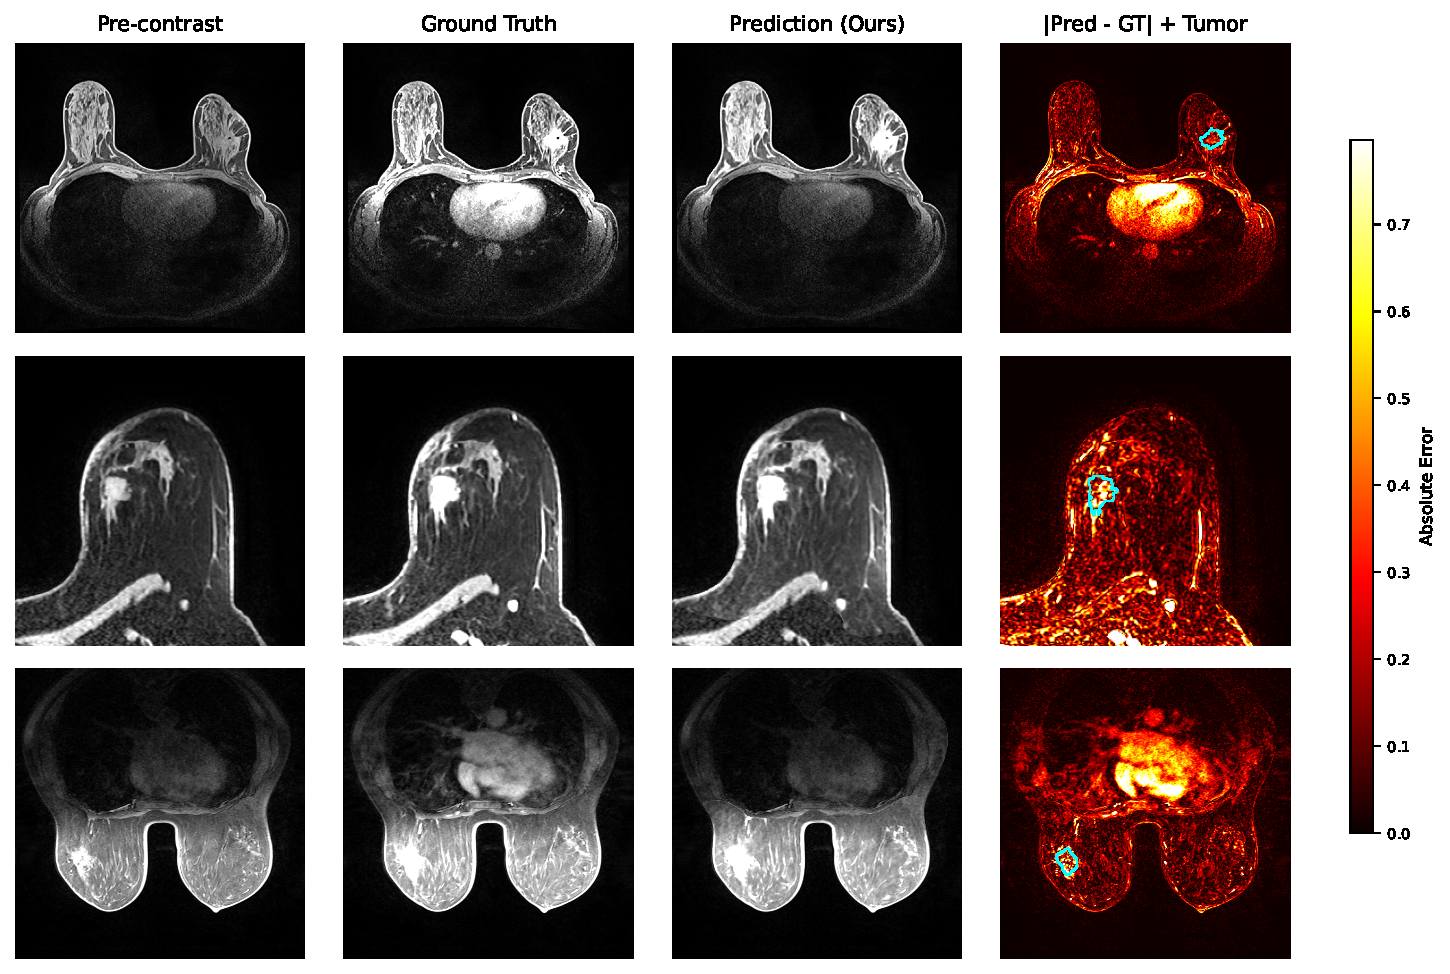
\includegraphics[width=0.80\textwidth]{figures/qualitative.pdf}
\caption{Qualitative results on three test patients from different datasets. Top: DUKE, Middle: ISPY2, Bottom: YUNNAN. Columns: pre-contrast, ground truth, prediction, error map with tumor contour (cyan).}
\label{fig:qualitative}
\end{figure}

\section{Discussion and Conclusion}
We presented a tumor-aware conditional GAN for virtual contrast enhancement in breast MRI. Per-image normalization provides a 25\% LPIPS improvement; the conditional tumor mask provides a 14\% Dice increase, addressing complementary failure modes.

A false positive in $m_t$ does not by itself produce a synthetic lesion, for two reasons. The generator is trained with \emph{predicted} masks, so a fraction of the $m_t{=}1$ regions it saw during training carried no enhancement in $y$; it therefore learns to treat $m_t$ as a prior to be reconciled with the pre-contrast appearance rather than as an instruction. And in residual mode the identity map is free --- $\Delta{=}0$ reproduces $x$ exactly --- so any non-zero $\Delta$ must be earned against the masked $L_1$ and perceptual terms, which penalize enhancement wherever $y \approx x$. Together these bias the network towards modulating structure already visible in $x$ rather than inventing it in healthy-looking parenchyma. This is a bias, not a guarantee: adversarial training can still synthesize plausible texture, and clinical deployment would require a dedicated false-positive study.

\paragraph{Limitations.}
MSE is dominated by outliers, and the breast-masked training loss is mismatched with the full-image evaluation protocol. On the MSEC finding, we tested a single weight and a single formulation, so we cannot rule out that a smaller $\lambda_{MSEC}$ or a tumor-restricted variant would still help; nor does our result speak to the multi-parametric setting in which the loss was validated~\cite{yang2026miccai}. A weight sweep, model ensembling, and multi-resolution processing are left to future work.

\bibliographystyle{splncs04}
\bibliography{references}
\end{document}